\documentclass[letterpaper, oneside, 12pt]{article}
\usepackage{graphicx}
\usepackage{rotating}
\usepackage[american]{babel}

\selectlanguage{american}

\newcommand{\ie}{i.e.,}
\newcommand{\eg}{e.g.,}


% document
\begin{document}

%\begin{titlepage}
\hspace{-7mm}
\begin{minipage}{\textwidth}
\begin{center}
\vspace{.5cm}
{\huge \bf Software Design Document\\[1.5ex]}
{\large \bf for a specific implementation of `BCI2000'}
\\[1.5cm]
{\Large Gerwin Schalk\\}
{\Large Thilo Hinterberger\\}
{\Large Dennis J. McFarland\\[1.5cm]}
%
\begin{minipage}{13cm}
  \begin{minipage}[c]{13cm}
    \begin{center}
      {\Large \bf New York State Department of Health\\[2ex]}
      {\large \bf Wadsworth Center\\[0.5ex]
       Laboratory of Nervous Systems Disorders\\[4ex]}
      {\Large \bf Eberhard--Karls--Universit\"at T\"ubingen\\[2ex]}
      {\large \bf Medizinische Fakult\"at\\[0.5ex]
       Institut f\"ur Medizinische Psychologie\\[0.5ex]}
    \end{center}
  \end{minipage}
  \\[1.0cm]
  \begin{minipage}[c]{6cm}
    \centerline{
\includegraphics{figures/DOHlogo}}
  \end{minipage}
  \hspace{1.5cm}
  \begin{minipage}[c]{3cm}
    \centerline{
\includegraphics{figures/EKUlogo}}
  \end{minipage}
\end{minipage}
%
\\[0.5cm]
\textbf{Sponsors} \\
\textit{Jonathan R. Wolpaw and Niels Birbaumer}
\\[1.0cm]
{Albany, NY} \\[1ex]
{February 2000--May 2001}
\\[1ex]Updated May 2003, J\"urgen Mellinger
\end{center}
\end{minipage}
\end{titlepage}

\title{Neuroscan Support in BCI2000}
\author{Gerwin Schalk\\ \small{\copyright{} 2004 Wadsworth Center, New York State Department of Health}\\ \small{supported by work from J\"{u}rgen Mellinger}\\ \small{Eberhard Karls University of T\"{u}bingen, Germany}}
\maketitle

\tableofcontents

\newpage

%\begin{abstract}
%\end{abstract}

\section{Introduction}

\sloppypar \emph{NuAmps/SynAmps} are EEG recording systems from Neuroscan, Inc., that are 
widely used in clinical settings. The increasing use of BCI2000 in those 
environments created the need for Neuroscan support in BCI2000. This document 
describes this support that consists of two components: A BCI2000-compatible 
Source Module (\texttt{Neuroscan.exe}) and a command-line tool 
(\texttt{neurogetparams}). These components are described below and have been 
tested with \emph{Neuroscan Acquire} version 4.3.1.

%\section{Background}
%As many other clinical systems, Neuroscan devices amplify and digitize signals 
%in a box outside of a computer, and then transmit these signals using a 
%proprietary and undocumented protocol to a computer.

\section{Neuroscan Source Module}

The BCI2000-compatible Source Module \texttt{Neuroscan.exe} can be used instead 
of any other source module. In addition to standard parameters (\ie{} 
\emph{SampleBlockSize}, \emph{SamplingRate}, \emph{SoftwareCh}), it only 
requests one Neuroscan-specific parameter (\emph{ServerAddress}) that defines 
the IP address (or host name) and the port number of the \emph{Acquire} server. 
An example for an appropriate definition is \texttt{localhost:3999}. Before 
starting BCI2000, you need to start \emph{Acquire}, click on the \emph{S} symbol 
in the top right corner (to enable the server) and start the server on any port. 
Please note that by default, \emph{Acquire} suggests port 4000, which is a port 
used by BCI2000. You might use port 3999 instead. Once the server is running, 
you can start BCI2000. It is imperative that certain parameters (\eg{} the 
number of channels) in BCI2000 match the settings in \emph{Acquire}. You can 
read these settings from \emph{Acquire} using the command line tool described in 
the following section. This command line tool can create a parameter file 
fragment that needs to be loaded on top of an existing parameter file every time 
a setting in \emph{Acquire} is changed.

\section{The \texttt{neurogetparams} Command Line Tool}

This command line tool reads system settings from the \emph{Neuroscan Acquire} 
server, displays them on a screen and creates a BCI2000 parameter file fragment 
if desired. It can be used as follows: \texttt{neurogetparams -address 
localhost:3999 -paramfile test.prm}. (The \emph{Acquire} server has to be 
enabled before using this tool.) Once BCI2000 is configured correctly, this 
parameter file fragment needs to be loaded on top of the existing configuration 
to make sure that the settings match. You only need to repeat this procedure if 
you change settings in \emph{Acquire} (\eg{} such as the number of channels or 
the amplification).

\begin{verbatim}
BCI2000 Parameter Tool for Neuroscan Acquire V4.3
*******************************************************************
(C)2004 Gerwin Schalk and Juergen Mellinger
        Wadsworth Center, New York State Dept of Health, Albany, NY
        Eberhardt-Karls University of Tuebingen, Germany
*******************************************************************
Signal Channels: 32
Event Channels:  1
Block Size:      40
Sampling Rate:   1000
Bits/Sample:     16
Resolution:      0.168uV/LSB
Parameter file test.prm successfully written
\end{verbatim}


\section{Undocumented Communication}

\emph{Neuroscan Acquire} supports communication options that are not documented 
in the \texttt{NetAcquire.doc} document. BCI2000 needs to use two of them, the 
request for basic Neuroscan configuration information (which will return 
information such as the number of channels and the sampling rate) and the 
receipt of packets of data, to function properly. They are listed below:\\

\begin{tabular}{|l|l|l|l|}
 \hline
 \textbf{Packet ID} & \textbf{Code} & \textbf{Request}   & \textbf{Body Size} \\
 \hline
 \hline
 "CTRL"   & 3 (Client Ctrl Code)    & 5 (Req Basic Info) & 0\\
 "DATA"   & 1 (Datatype Info)       & 3 (InfoType BasicInfo) & bodyLen \\
 "DATA"   & 2 (EEG Data)            & 1 (Raw 16-bit)     & bodyLen \\
 \hline
\end{tabular}

\subsection{Request Basic Information}

The client sends a request for basic information ("CTRL", Client Ctrl Code, Req 
Basic Info). The server responds by sending a data block ("DATA", Datatype Info, 
InfoType BasicInfo) that contains a data structure describing the current 
configuration of data acquisition in Acquire. This data structure is as follows:

\begin{verbatim}
struct AcqBasicInfo
 {
 DWORD dwSize;      // Size of structure, used for version control
 int   nEegChan;    // Number of EEG channels
 int   nEvtChan;    // Number of event channels
 int   nBlockPnts;  // Samples in block
 int   nRate;       // Sampling rate (in Hz)
 int   nDataSize;   // 2 for "short", 4 for "int" type of data
 float fResolution; // Resolution for LSB
 };
\end{verbatim}

The first element, dwSize, can and should be cross checked with the length of 
the structure \texttt{AcqBasicInfo} and must match.

\subsection{Receive 16-bit Data Packet}

The client may send a \emph{Request to Start Sending Data} to the Acquire server 
(as described in the \texttt{NetAcquire.doc} document). This will prompt the 
server to start sending blocks of raw signal values. In order to interpret these 
signal values, the client must first have sent a \emph{Request for Basic 
Information}, as described above. The incoming data packets ("DATA", EEG Data, 
Raw 16-bit) can then be interpreted using this information and the code below.

\begin{verbatim}
// make sure the body has the right length
assert((int)(pMsg->m_dwSize) == 
              (int)(m_BasicInfo.nEegChan+m_BasicInfo.nEvtChan)
              *m_BasicInfo.nBlockPnts*m_BasicInfo.nDataSize);
// process raw 16 bit data
for (int samp=0; samp<m_BasicInfo.nBlockPnts; samp++)
 {
 for (int ch=0; ch<m_BasicInfo.nEegChan+m_BasicInfo.nEvtChan; ch++)
  {
  short *sample=(short *)pMsg->m_pBody;
  printf("%d ", sample[samp*(m_BasicInfo.nEegChan+m_BasicInfo.nEvtChan)+ch]);
  }
 }
\end{verbatim}


%\begin{figure}[ht]
% \centerline{\scalebox{1}{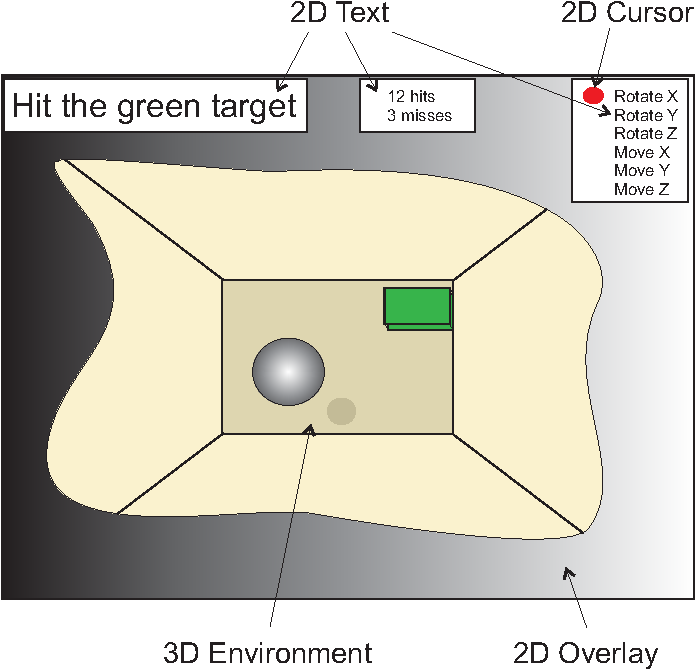
\includegraphics{figure/environment.pdf}}}
% \caption{Graphical Environment.}
% \label{fig:environment}
%\end{figure}


\end{document}

